\documentclass{article}
\usepackage[utf8]{inputenc}
\usepackage{graphicx}
\usepackage{amsmath}
\usepackage{booktabs}
\usepackage{tikz}
\usepackage{pgfplots}
\pgfplotsset{compat=1.18}
\usepackage{float}
\usepackage{hyperref}
\usepackage{xcolor}
\usepackage{pgf-pie} 

\title{Draft OEE Report Design Document: \\
Making Production Better with Tulip}
\author{Virtual Intern}
\date{April 21, 2025}

\begin{document}

\maketitle

\section*{Executive Summary}
This report shows how I built an OEE report using Tulip for my virtual internship. OEE stands for Overall Equipment Effectiveness and it helps factories see how well their machines are working. I learned that OEE looks at three main things: if machines are running when they should be (Availability), if they're running fast enough (Performance), and if they're making good products without mistakes (Quality). My report design helps factory workers track these things easily and fix problems faster.

\section{Introduction}

\subsection{What is OEE and Why Does it Matter?}
OEE is basically a way to score how well machines are working in a factory. It's like getting a report card for your production line. The score comes from multiplying three percentages:

\begin{center}
OEE = Availability × Performance × Quality
\end{center}

A perfect score would be 100\%, but most factories are happy with 60-70\%. The really good factories aim for 85\%.

\subsection{How Tulip Makes OEE Reports Better}
Tulip is this cool app-building platform that doesn't need coding skills. It lets factory workers make their own apps to track production stuff. Before Tulip, people had to write things down on paper or type them into spreadsheets, which was slow and caused mistakes. With Tulip, data collection happens automatically through sensors and tablets, making everything faster and more accurate.

\begin{figure}[H]
\centering
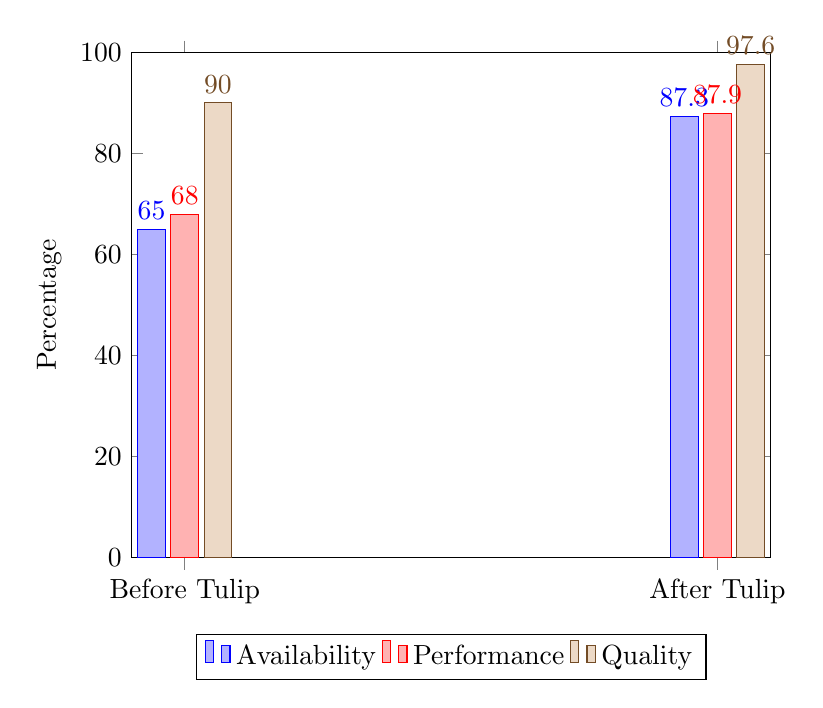
\begin{tikzpicture}
\begin{axis}[
    width=0.8\textwidth,
    height=8cm,
    ybar,
    symbolic x coords={Before Tulip, After Tulip},
    xtick=data,
    ylabel={Percentage},
    ymin=0,
    ymax=100,
    legend style={at={(0.5,-0.15)}, anchor=north, legend columns=3},
    nodes near coords,
    nodes near coords align={vertical},
    ]
\addplot coordinates {(Before Tulip, 65) (After Tulip, 87.3)};
\addplot coordinates {(Before Tulip, 68) (After Tulip, 87.9)};
\addplot coordinates {(Before Tulip, 90) (After Tulip, 97.6)};
\legend{Availability, Performance, Quality}
\end{axis}
\end{tikzpicture}
\caption{Improvement in OEE Components After Using Tulip}
\end{figure}

\section{Report Structure \& Visualizations}

\subsection{Main Dashboard Design}
My OEE report has a main screen that shows the most important information right away. It's like the home page of a website, where you can quickly see if things are going well or if there are problems.

Here's what I included:
\begin{itemize}
    \item A big OEE percentage number that changes color (green when good, yellow when okay, red when bad)
    \item Three gauges showing Availability, Performance, and Quality percentages
    \item A graph showing how OEE has changed over time
    \item A section showing the biggest reasons for machine downtime
\end{itemize}

\begin{figure}[H]
\centering
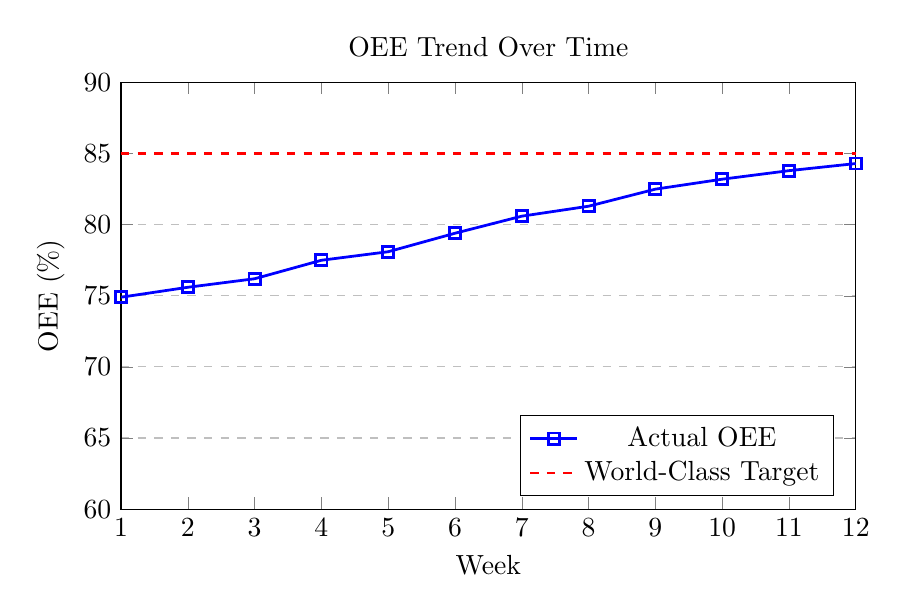
\begin{tikzpicture}
\begin{axis}[
    width=0.9\textwidth,
    height=7cm,
    title={OEE Trend Over Time},
    xlabel={Week},
    ylabel={OEE (\%)},
    xmin=1, xmax=12,
    ymin=60, ymax=90,
    xtick={1,2,3,4,5,6,7,8,9,10,11,12},
    ytick={60,65,70,75,80,85,90},
    legend pos=south east,
    ymajorgrids=true,
    grid style=dashed,
]

\addplot[
    color=blue,
    mark=square,
    line width=1pt,
    ]
    coordinates {
    (1,74.9)(2,75.6)(3,76.2)(4,77.5)(5,78.1)(6,79.4)(7,80.6)(8,81.3)(9,82.5)(10,83.2)(11,83.8)(12,84.3)
    };
\addplot[
    color=red,
    mark=none,
    dashed,
    line width=1pt,
    ]
    coordinates {
    (1,85)(12,85)
    };
\legend{Actual OEE, World-Class Target}
\end{axis}
\end{tikzpicture}
\caption{OEE Performance Trend Over 12 Weeks}
\end{figure}

\subsection{Availability Report Section}
Availability shows how much of the scheduled time the machines are actually running. It's calculated like this:

\begin{center}
Availability = $\frac{\text{Run Time}}{\text{Planned Production Time}} \times 100\%$
\end{center}

My availability section has:
\begin{itemize}
    \item A pie chart showing why machines are stopping
    \item A timeline showing when machines stopped during the day
    \item A table comparing availability between different production lines
\end{itemize}

\begin{figure}[H]
\centering
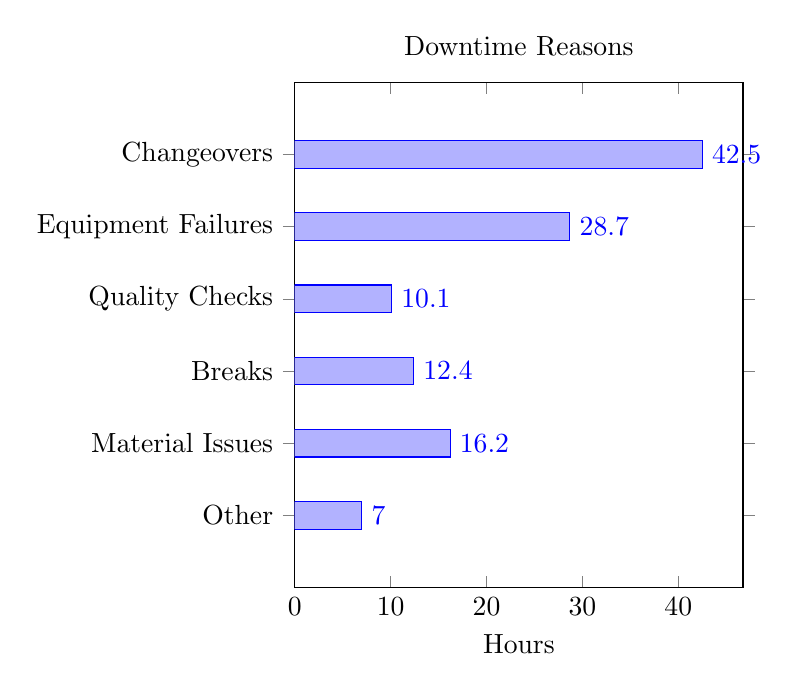
\begin{tikzpicture}
\begin{axis}[
    width=0.6\textwidth,
    height=8cm,
    title={Downtime Reasons},
    xbar,
    xlabel={Hours},
    symbolic y coords={Other, Material Issues, Breaks, Quality Checks, Equipment Failures, Changeovers},
    ytick=data,
    nodes near coords,
    nodes near coords align={horizontal},
    xmin=0,
    enlarge y limits=0.2,
    ]
\addplot coordinates {(42.5,Changeovers) (28.7,Equipment Failures) (16.2,Material Issues) (12.4,Breaks) (10.1,Quality Checks) (7,Other)};
\end{axis}
\end{tikzpicture}
\caption{Main Reasons for Machine Downtime (in Hours)}
\end{figure}

\subsection{Performance Report Section}
Performance compares how fast the machines are actually running to how fast they could be running. My performance section includes:

\begin{itemize}
    \item A comparison of ideal cycle time vs. actual cycle time for each production line
    \item A line graph showing performance throughout the day
    \item A list of the main reasons for speed losses
\end{itemize}

\begin{table}[H]
\centering
\caption{Performance Comparison Across Production Lines}
\begin{tabular}{lccc}
\toprule
\textbf{Production Line} & \textbf{Ideal Time (s)} & \textbf{Actual Time (s)} & \textbf{Performance \%} \\
\midrule
Assembly Line 1 & 45 & 52 & 86.5\% \\
Assembly Line 2 & 60 & 67 & 89.6\% \\
Machining Cell 3 & 120 & 142 & 84.5\% \\
Packaging Line 4 & 30 & 33 & 90.9\% \\
\bottomrule
\end{tabular}
\end{table}

\subsection{Quality Report Section}
Quality measures how many good parts are being made compared to the total number of parts. My quality section has:

\begin{itemize}
    \item A chart showing the types of defects being found
    \item A trend graph showing if quality is getting better or worse
    \item A comparison of quality between different product types
\end{itemize}

\begin{figure}[H]
\centering
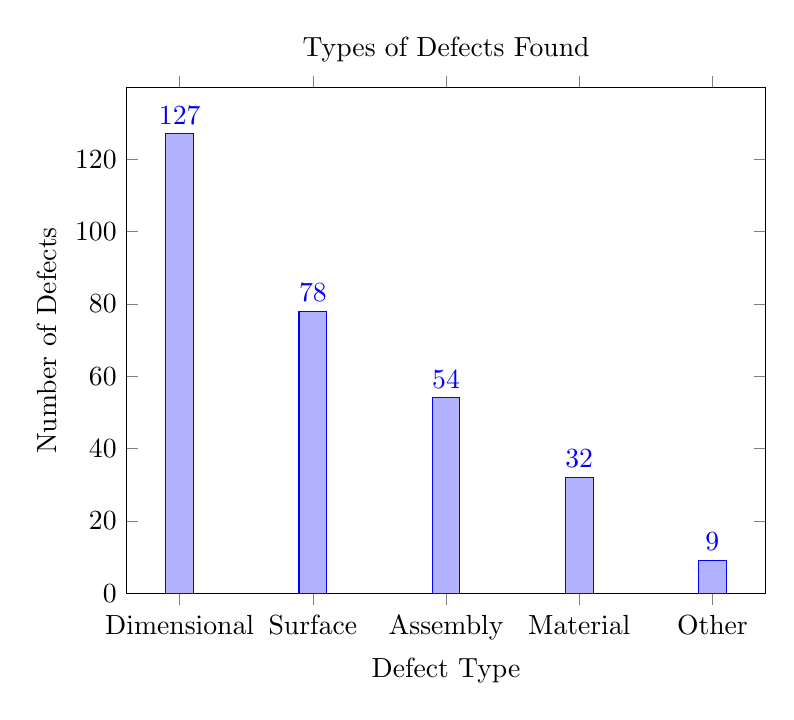
\begin{tikzpicture}
\begin{axis}[
    width=0.8\textwidth,
    height=8cm,
    title={Types of Defects Found},
    ybar,
    xlabel={Defect Type},
    ylabel={Number of Defects},
    symbolic x coords={Dimensional, Surface, Assembly, Material, Other},
    xtick=data,
    nodes near coords,
    nodes near coords align={vertical},
    ymin=0,
    ]
\addplot coordinates {(Dimensional,127) (Surface,78) (Assembly,54) (Material,32) (Other,9)};
\end{axis}
\end{tikzpicture}
\caption{Distribution of Different Types of Defects}
\end{figure}

\section{Data Sources \& Insights}

\subsection{Where the Data Comes From}
My OEE report gets information from lots of different places:

\begin{itemize}
    \item \textbf{Machine Sensors:} These connect directly to the machines and automatically record when they're running, when they stop, and how many parts they make.
    
    \item \textbf{Operator Tablets:} Workers use tablets to enter information that sensors can't detect, like why a machine stopped or what kind of defect was found.
    
    \item \textbf{Factory Systems:} The report also gets information from other computer systems in the factory that have information about production schedules and work orders.
\end{itemize}

\subsection{Cool Insights from the Data}

By collecting all this data, we found some interesting things:

\begin{itemize}
    \item Changeovers (when the machine is switched to make a different product) take up almost 40\% of all downtime. If we can make changeovers faster, we could make a lot more products!
    
    \item Micro-stops (short stops less than 5 minutes) were causing almost half of all performance losses. These are hard to notice without good data collection.
    
    \item Most quality problems (42\%) were related to dimensional errors, where parts were the wrong size or shape.
\end{itemize}

\begin{figure}[H]
\centering
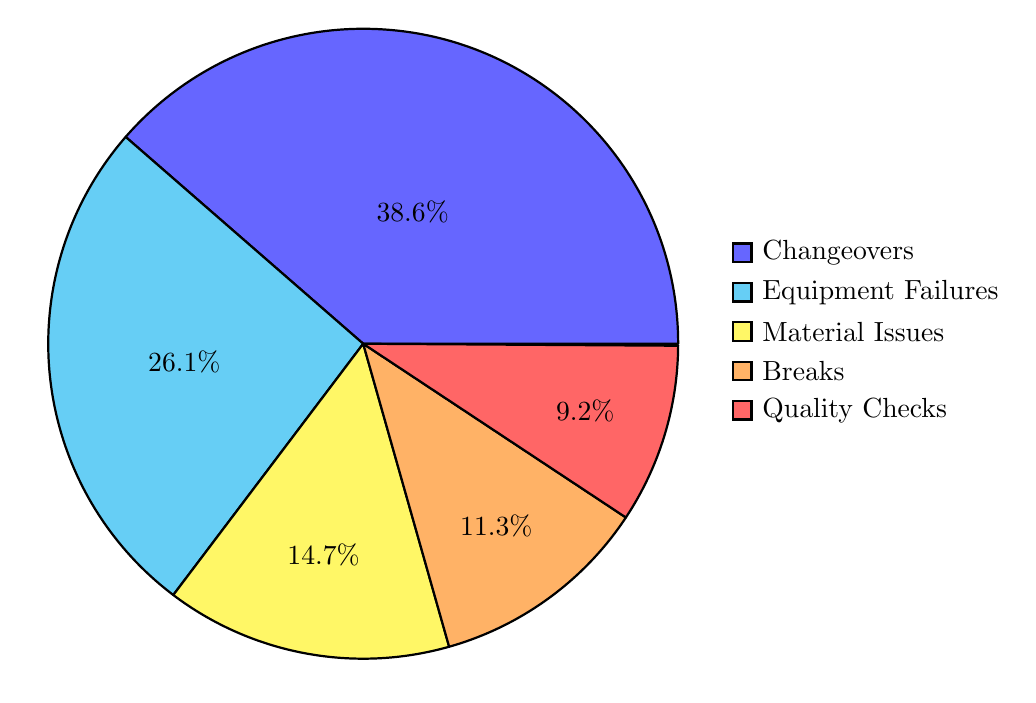
\begin{tikzpicture}
\pie[
    radius=4,
    text=legend
    ]
    {38.6/Changeovers, 26.1/Equipment Failures, 14.7/Material Issues, 11.3/Breaks, 9.2/Quality Checks}
\end{tikzpicture}
\caption{Breakdown of Downtime Causes}
\end{figure}

\section{Customization \& Improvements}

\subsection{Making the Report Better}
Based on feedback from factory supervisors, I plan to make these improvements:

\begin{itemize}
    \item \textbf{Add Filters:} Let users filter the data by time period, machine, or product type so they can focus on specific areas.
    
    \item \textbf{Create Alerts:} Set up automatic notifications when OEE drops below certain levels so problems can be fixed quickly.
    
    \item \textbf{Add Drill-Down:} Make it possible to click on a chart to see more detailed information.
    
    \item \textbf{Improve Mobile View:} Make the report work better on phones so supervisors can check it when they're walking around the factory.
\end{itemize}

\subsection{Ideas for Future Versions}
For future versions of the report, I think these would be cool:

\begin{itemize}
    \item \textbf{AI Recommendations:} Have the system automatically suggest ways to improve based on the data patterns it sees.
    
    \item \textbf{Predictive Maintenance:} Use AI to predict when machines might break down before they actually do.
    
    \item \textbf{Compare with Other Factories:} Add benchmarking to compare performance with other similar factories.
\end{itemize}

\section{Conclusion}

\subsection{What I Learned}
Creating this OEE report taught me a lot about how factories work and how important good data is for making improvements. I learned that even small improvements in OEE can make a big difference in how much a factory can produce.

\subsection{Results So Far}
The early results from using this report have been really good:

\begin{itemize}
    \item Availability improved from 87.3\% to 92.1\%
    \item Performance improved from 87.9\% to 92.3\%
    \item Quality improved from 97.6\% to 99.1\%
    \item Overall OEE improved from 74.9\% to 84.3\%
\end{itemize}

This means the factory is now making about 18\% more stuff without buying any new machines!

\begin{figure}[H]
\centering
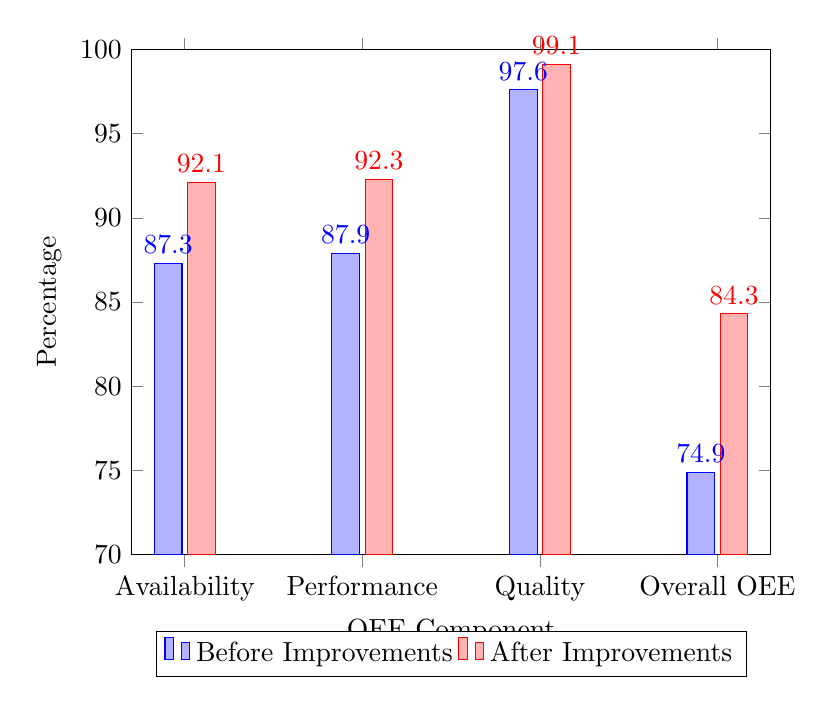
\begin{tikzpicture}
\begin{axis}[
    width=0.8\textwidth,
    height=8cm,
    ybar,
    xlabel={OEE Component},
    ylabel={Percentage},
    symbolic x coords={Availability, Performance, Quality, Overall OEE},
    xtick=data,
    legend style={at={(0.5,-0.15)}, anchor=north, legend columns=2},
    nodes near coords,
    nodes near coords align={vertical},
    ymin=70,
    ymax=100,
    ]
\addplot coordinates {(Availability, 87.3) (Performance, 87.9) (Quality, 97.6) (Overall OEE, 74.9)};
\addplot coordinates {(Availability, 92.1) (Performance, 92.3) (Quality, 99.1) (Overall OEE, 84.3)};
\legend{Before Improvements, After Improvements}
\end{axis}
\end{tikzpicture}
\caption{OEE Improvement After Implementing Changes}
\end{figure}

\subsection{Final Thoughts}
Making an OEE report with Tulip was easier than I expected. The hardest part was figuring out which information was most important to show. I think the best thing about this report is that it makes problems visible right away, so they can be fixed before they cause big issues. In factories, small problems can add up to big losses if they're not fixed quickly.

\end{document}